{\bf An overview of Sections \ref{sec:BandVan}-\ref{sec:mod8}}
This and the following two sections are devoted to the proof of \Cref{thm:mod8}, which will be proven as \Cref{thm:mod8-main-thm}. To prove \Cref{thm:mod8-main-thm}, we will show that there exists a line of slope $\frac{1}{5}$ on some finite page of the modified $\HFt$-Adams spectral sequence of the mod $8$ Moore spectrum $C(8)$ above which the only classes are those detecting the $K(1)$-local homotopy of $C(8)$.\footnote{For the notion of a modified Adams spectral sequence, see \cite[Section 3]{BHHM}.}

In this section, we will axiomatize this property into the defintion of a $v_1$-banded vanishing line on a synthetic spectrum. We will then show that the property of having a $v_1$-banded vanishing line is generic, i.e. is closed under retractions, bigraded suspensions and cofiber sequences of synthetic spectra. In \Cref{sec:Y}, we will show that $\nu_{\HFt} (Y) = \nu_{\HFt} (C(2) \otimes C(\eta))$ admits a $v_1$-banded vanishing line.
In \Cref{sec:mod8}, we will establish a $v_1$-banded vanishing line on $C(\wt{8})$ and use this line to prove \Cref{thm:mod8-main-thm}.\footnote{The synthetic spectrum $C(\wt{8})$ is defined in \Cref{sec:mod8}. It encodes the modified $\HFt$-Adams spectral sequence of $C(8)$.}  The proof of the $v_1$-banded vanishing line of $C(\wt{8})$ is a genericity argument, building from the case of $\nu_{\HFt} (Y)$. As in Sections \ref{sec:AppendixVL} and \ref{sec:ANvl}, we will sedulously keep track of intercepts and torsion levels throughout.
%
%The key point is to show that there exists a large gap at some finite page of the $\HFt$-Adams spectral sequence between the $K(1)$-local classes in $\pi_* (C(8))$ and the rest of the homotopy of $C(8)$. More precisely, we will establish the existence of a line of slope $\frac{1}{5}$ in the $\mathrm{E}_{\infty}$-page of the $\mathrm{H}\F_2$-Adams spectral sequence of the mod $8$ Moore spectrum $C(8)$ above which every class is detected in the $K(1)$-localization $L_{K(1)} C(8)$. We will prove this by a genericity argument. 
%
%In this section, we formulate in \Cref{dfn:banded-vanishing-line} the notion of a $v_1$-banded vanishing line and show in \Cref{prop:band-in-cofiber-seqs} that the existence of such a line is is closed under cofibers in the category of synthetic spectra. In \Cref{sec:Y}, we will prove that $\nu_{\HFt}( C(2) \otimes C(\eta) )$ admits a $v_1$-banded vanishing line of slope $\frac{1}{5}$, and in \Cref{sec:mod8} we will use \Cref{prop:band-in-cofiber-seqs} to deduce that $C(\wt{2}^3)$ does as well, where $\wt{2}: \Ss^{1,2} \to \Ss^{0,0}$ is as in \Cref{prop:syn-toda-range}. This will imply the existence of the desired line of slope $\frac{1}{5}$ in the $\mathrm{H}\F_2$-Adams spectral sequence for $C(8)$. We begin with a few preliminary definitions.

\begin{dfn}
    Given a $\Z[\tau]$-module $M$, we let $M_{\mathrm{tor}} \subset M$ denote the subgroup of $\tau$-power torsion elements and $M_{\mathrm{tf}}$ the torsion free quotient $M / M_{\mathrm{tor}}$. When there are other subscripts present, we will sometimes find it convenient to write $M^{\mathrm{tor}}$ and $M^{\mathrm{tf}}$ in place of $M_{\mathrm{tor}}$ and $M_{\mathrm{tf}}$, respectively.
\end{dfn}

\begin{dfn}\label{dfn:synth-filt}
    Given a synthetic spectrum $X$, we let $F^s \pi_{k} (\tau^{-1} X) \subset \pi_{k} (\tau^{-1} X)$ denote the image of $\pi_{k,k+s} X \to \pi_{k} (\tau^{-1} X)$. This defines a descending filtration on $\pi_k (\tau^{-1} X)$, which is natural in $X$.
\end{dfn}

\begin{rmk}
  The natural map $\pi_{k,k+s} (X)_{\mathrm{tf}} \to F^s \pi_k (\tau^{-1} X)$ is an isomorphism.
\end{rmk}

\begin{rmk}
    Let $Y$ be a $E$-nilpotent complete spectrum whose $E$-Adams spectral sequence converges strongly. By \Cref{cor:synth-filt}, the filtration $F^s \pi_k (\tau^{-1} \nu_E (Y))$ coincides with the $E$-Adams filtration on $\pi_k (Y) \cong \pi_k (\tau^{-1} \nu_E (Y))$.
\end{rmk}

\begin{cnv}
    In the remainder of this section, we will fix a prime $p$ and work exclusively with the category $\mathrm{Syn}_{\HFp}$ of synthetic spectra with respect to $\HFp$.
\end{cnv}

\begin{dfn}\label{dfn:banded-vanishing-line}
  We say that a synthetic spectrum $X$ has a $v_1$-banded vanishing line with
  \begin{itemize}
  \item band intercepts $b \leq d$
  \item range of validity $v$
  \item line of slope $m < \frac{1}{2p-2}$ and intercept $c$
  \item torsion bound $r$
  \end{itemize}
  if the following conditions hold:
  \begin{enumerate}
  \item every class in $\pi_{k,k+s} (X)_{\mathrm{tor}}$ is $\tau^{r}$-torsion for $s \geq mk+c$ and $k \geq v$,
  \item the natural map
    $$ F^{\frac{1}{2p-2} k + b} \pi_k (\tau^{-1} X) \to F^{mk + c} \pi_k (\tau^{-1} X) $$
    is an isomorphism for $k \geq v$,
  \item the composite
    $$ F^{\frac{1}{2p-2} k + b} \pi_{k} (\tau^{-1} X) \to \pi_k(\tau^{-1}X) \to \pi_k (L_{K(1)} \tau^{-1} X) $$
    is an equivalence for $k \geq v$,
  \item $\pi_{k,k+s} (X) = 0$ for $s > \frac{1}{2p-2} k + d$.
  \end{enumerate}
  
  More concisely, we will say that that $X$ has a $v_1$-banded vanishing line with parameters $(b \leq d, v, m, c, r)$.
\end{dfn}

%% \begin{rmk} \label{rmk:bvl-convexity}
%%   \todo{Comment on the convexity properties of this definition. AS: I don't really want to write this remark... Robert can write it if he feels strongly about it.}
%% \end{rmk}

\begin{rmk}
  Given an $\HFp$-nilpotent complete spectrum $X$, we will say that the $\HFp$-Adams spectral sequence of $X$ admits a $v_1$-banded vanishing line with parameters $(b \leq d, v, m, c, r)$ if $\nu_{\HFp} (X)$ admits one. This is justified by the following proposition:
\end{rmk}

\begin{prop} \label{prop:banded-adams}
    Given an $\HFp$-nilpotent complete spectrum $X$, $\nu_{\HFp} (X)$ admits a $v_1$-banded vanishing line with parameters $(b \leq d, v, m, c, r)$ if and only if the $\HFp$-based Adams spectral sequence for $X$ satisfies the following conditions:
    \begin{enumerate}
        \item[($1'$)] $\mathrm{E}_{r+2} ^{s,k+s} = \mathrm{E}_{\infty} ^{s,k+s}$ for $s \geq mk+c$ and $k \geq v$.
        \item[($2'$)] $\mathrm{E}_{r+2} ^{s,k+s} = 0$ for $mk+c \leq s < \frac{1}{2p-2}k + b$ and $k \geq v$.
        \item[($3'$)]$F^{\frac{1}{2p-2} k + b} \pi_k (X) \to \pi_k (L_{K(1)} X)$ is an isomorphism for $k \geq v$, where $F$ is the $\HFp$-Adams filtration.
        \item[($4'$)] $\mathrm{E}_2 ^{s,k+s} = 0$ for all $s > \frac{1}{2p-2}k+d$.
    \end{enumerate}
\end{prop}

\begin{proof}
    It follows from \Cref{lemm:vanishing-line-converge} and \Cref{lemm:vanishing-converge} that the $\HFp$-based Adams spectral sequence for $X$ converges strongly; therefore we may use \Cref{thm:synthetic-Adams} and its corollaries. By \Cref{prop:vanishing-line-Adams} we know that (4) and ($4'$) are equivalent. Using (4) to ground the induction started by \Cref{cor:tau-torsion-bound} we learn (1) and ($1'$) are equivalent. Using \Cref{cor:synth-filt} we may identify the filtration appearing in the definition of a banded vanishing line with the Adams filtration. This allows us to conclude that (2) and (3) are equivalent to ($2'$) and ($3'$), respectively.
\end{proof}

In \Cref{fig:banded} we use \Cref{prop:banded-adams} to illustrate the meaning of a banded vanishing line on $\nu X$. 
As we shall see, \Cref{dfn:banded-vanishing-line} captures the behavior of the modified Adams spectral sequence of a type $1$ spectrum. Moreover, it is formulated in such a way that it is a generic condition, i.e. the full subcategory of synthetic spectra satisfying \Cref{dfn:banded-vanishing-line} for a fixed $m$ and varying $(b \leq d, v, c, r)$ is closed under retracts, bigraded suspensions and cofiber sequences. We prove this genericity in \Cref{lemm:band-retract-susp} and \Cref{prop:band-in-cofiber-seqs}. A key feature of our approach is that we keep explicit track of how the constants $(b \leq d, v, c, r)$ change under retracts, bigraded suspensions and cofiber sequences.

\begin{figure}
  \centering
    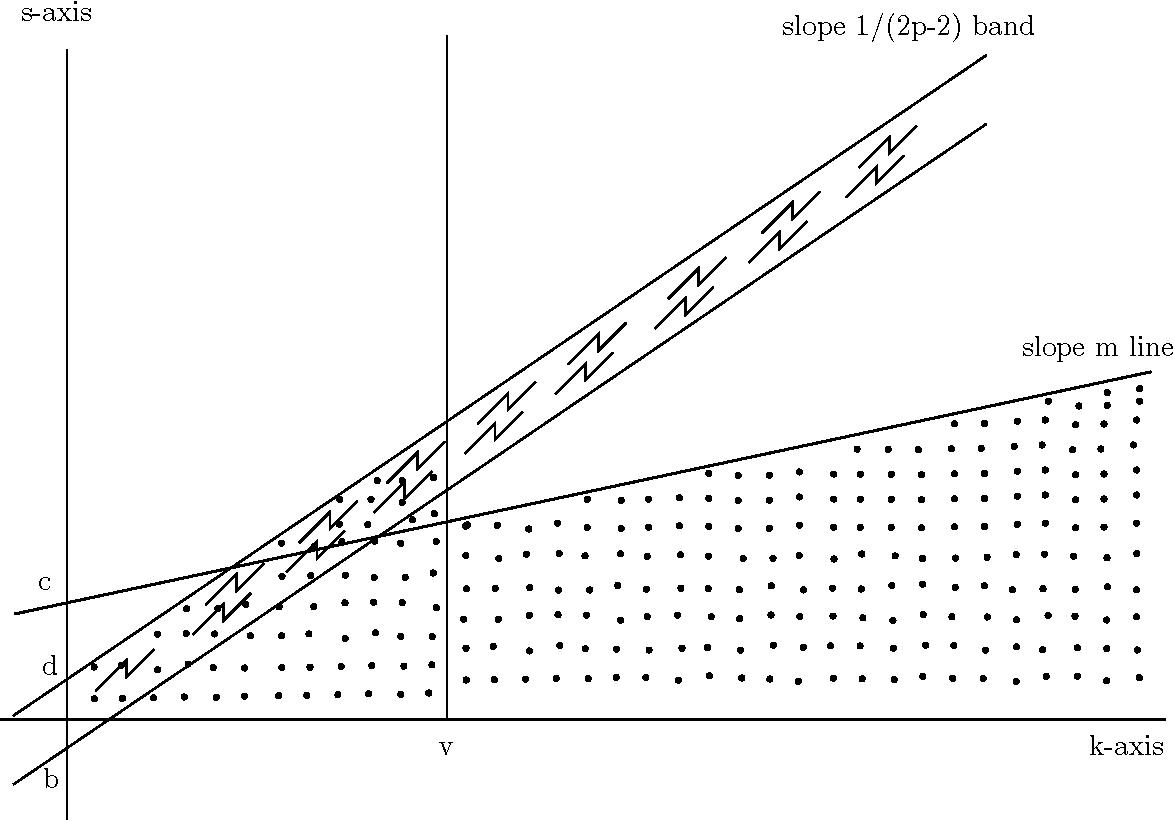
\includegraphics[scale=0.6]{banded-diagram-cm.pdf}
    \caption{In this figure we display a picture of what the $\mathrm{E}_{r+2}$-page of the $\HFp$-Adams spectral sequence of an $\HFp$-nilpotent complete spectrum that admits an $v_1$-banded vanishing line with parameters $(b \leq d, v, m, c, r)$ might look like. We highlight the following features:\\
      (1) The top region is already empty at the $E_2$-page. \\
      (2) The region indicated with lightning flashes is the band (it is depicted this way since this is how it appears for $\Ss/2$) and contains all classes detected $K(1)$-locally. \\
      (3) The empty region below the band vanishes by the $E_{r+2}$-page. \\
      (4) In the dotted region no conditions are imposed.}
    \label{fig:banded}
\end{figure}

%Let's unpack the meaning of \Cref{dfn:banded-vanishing-line} in the case of $X = \nu_E (Y)$. to $X$ converging to the homotopy of $\tau^{-1} X$, which by \Cref{.} \todo{Cite result connecting ASS and $\tau$-bockstein here.} is the Adams spectral sequence when $X = \nu (Y)$ for a spectrum $Y$. The following statements are only asked to hold in the range of validity, i.e. for stems in degree at least $v$.
%
%Part (1) of the definition states that the spectral sequence collapses above the line of slope $m$ and intercept $c$ at finite page $E_{r +2}$. Part (2) of the definition states that every infinite cycle above the line of slope $m$ and intercept $c_X$ in fact lives above a line of slope $q^{-1}$ and intercept $b_X$. Part (4) implies that there is a vanishing line of slope $q^{-1}$ and intercept $d_X$ at the $E_2$-page, so that in fact the classes mentioned in part (2) lie along the vanishing line. Finally, part (3) asks that the classes lying along the vanishing line are exactly the $K(1)$-local classes.


\begin{exm} \label{exm:miller-banded}
    The main result of \cite{Miller} implies that the $\HFp$-Adams spectral sequence for the mod $p$ Moore spectrum $C(p)$ admits a $v_1$-banded vanishing line of slope $\frac{1}{p^2-p-1}$ for $p$ odd. In \Cref{sec:Y}, we will show that the methods of \cite{Miller} may also be used to obtain a $v_1$-banded vanishing line of slope $\frac{1}{5}$ in the $\HFt$-Adams spectral sequence of $Y = C(2) \otimes C(\eta)$.
\end{exm}

We begin with the behavior of \Cref{dfn:banded-vanishing-line} under retracts and suspensions.

\begin{lem}[Banded Genericity (part 1)] \label{lemm:band-retract-susp}
  Suppose that a synthetic spectrum $X$ has a $v_1$-banded vanishing line with parameters $(b \leq d, v, m, c, r)$. Then
  \begin{enumerate}
  \item any retract of $X$ has a $v_1$-banded vanishing line with the same parameters as $X$,
  \item $\Sigma^{k,k} X$ has a $v_1$-banded vanishing line with parameters
    $$ \left( b - \frac{1}{2p-2} k \leq d - \frac{1}{2p-2} k, v + k, m, c - mk, r \right), $$
  \item $\Sigma^{0,s} X$ has a $v_1$-banded vanishing line with parameters
    $$ ( b + s \leq d + s, v, m, c + s, r). $$
  \end{enumerate}
\end{lem}

\begin{proof}
  This lemma is a version of \Cref{lemm:suspension-line} for banded vanishing lines.
  As with the earlier lemma it follows from tracking how bigraded homotopy groups change under retracts and bigraded suspensions.
\end{proof}


\begin{prop}[Banded Genericity (part 2)] \label{prop:band-in-cofiber-seqs}
  Let $A \xrightarrow{f} B \xrightarrow{g} C \xrightarrow{\delta} \Sigma A$ be a cofiber sequence of synthetic spectra such that
  \begin{itemize}
  \item $A$ has a $v_1$-banded vanishing line with parameters $(b_A \leq d_A, v_A, m, c_A, r_A)$ and
  \item $C$ has a $v_1$-banded vanishing line with parameters $(b_C \leq d_C, v_C, m, c_C, r_C)$.
  \end{itemize}
  Then, $B$ has a banded vanishing line with parameters $(b_B \leq d_B, v_B, m, c_B, r_B)$, where
  \begin{itemize}
  \item $b_B = \min(b_A, b_C - r_A) \leq \max(d_A, d_C) = d_B$,
  \item $v_B = \max(v_A + 1,v_C, \frac{c_B - b_B}{(2p-2)^{-1}-m})$,
  \item $c_B = \max(c_A + r_C, c_C)$,
  \item $r_B = r_A + \max \left( r_C, \left\lfloor \max(d_A, \min(d_A + r_C, d_C)) - b_C - \frac{1}{2p-2} \right\rfloor \right)$.
  \end{itemize}
\end{prop}

% Let us give names to the maps in our cofiber sequence as follows:
% $$ \Sigma^{-1,0} C \xrightarrow{\delta} A \xrightarrow{f} B \xrightarrow{g} C. $$
In order to prevent expressions such as $F^{\frac{1}{2p-2}k + b_A}\pi_k(\tau^{-1}A)$ from cluttering the proof of \Cref{prop:band-in-cofiber-seqs}, we introduce the following compact notation (which will not appear outside this section):
\begin{center}
  \begin{tabular}{cc cc cc}
    $\sampi \coloneqq (2p-2)^{-1}$ & $L \coloneqq L_{K(1)}$ &  
    $\bar{A} \coloneqq \tau^{-1}A$ & $\bar{B} \coloneqq \tau^{-1}B$ & $\bar{C} \coloneqq \tau^{-1}C$ \\
  \end{tabular}
\end{center}

Before starting the proof of \Cref{prop:band-in-cofiber-seqs}, we prove two lemmas:

\begin{lem}\label{lemm:lift-filt-bnd}
  Suppose that $A \xrightarrow{f} B \xrightarrow{g} C$ is a cofiber sequence of synthetic spectra,
  where every $\tau$-power torsion element of $\pi_{k,k+s} (C)$ is $\tau^{r}$-torsion.
  Then, the indicated lift exists in the diagram below:
\begin{center}
  \begin{tikzcd}
    F^s\pi_k(A) \ar[r, two heads] \ar[d, hook] &
    \mathrm{Im}(F^sf) \ar[r, hook] \ar[d, hook] &
    \ker(F^sg) \ar[r, hook] \ar[d, hook] \ar[dl, dashed] &
    F^s\pi_k(B) \ar[r] \ar[d, hook] &
    F^s\pi_k(C) \ar[d,hook] \\
    F^{s-r}\pi_k(A) \ar[r, two heads] &
    \mathrm{Im}(F^{s-r}f) \ar[r, hook]  &
    \ker(F^{s-r}g) \ar[r, hook]  &
    F^{s-r}\pi_k(B) \ar[r]  &
    F^{s-r}\pi_k(C)  
  \end{tikzcd}
\end{center}
\end{lem}

\begin{proof}
  Let $D_c$ denote the long exact sequence of bigraded homotopy groups for $A \to B \to C$ considered as an acyclic chain complex such that $\pi_{k,k+c}(B)$ is placed in degree zero. The complex $D_c$ fits into a level-wise short exact sequence $D_c^{\mathrm{tor}} \to D_c \to D_c^{\mathrm{tf}}$ where $D_c^{\mathrm{tor}}$ and $D_c^{\mathrm{tf}}$ are given by the same decorations applied level-wise. This lemma is equivalent to the statement that the map
  $$ H_0(D_s^{\mathrm{tf}}) \xrightarrow{\tau^r} H_0(D_{s-r}^{\mathrm{tf}}) $$
  is zero. Using the cofiber sequence of chain complexes above this map is isomorphic to the map
  $$ H_{-1}(D_s^{\mathrm{tor}}) \xrightarrow{\tau^r} H_{-1}(D_{s-r}^{\mathrm{tor}}). $$
  The latter map is zero because the map
  $$ \pi_{k,k+s}(C)_{\mathrm{tor}} \xrightarrow{\tau^r} \pi_{k,k+s-r}(C)_{\mathrm{tor}} $$
  is zero.
\end{proof}

\begin{lem} \label{lemm:qoppa-exactness}
  Under the hypotheses and notation of \Cref{prop:band-in-cofiber-seqs}, the sequence
  $$ F^{\qoppa -1} \pi_{k+1}(\bar{C}) \to F^\qoppa \pi_{k}(\bar{A}) \to F^\qoppa \pi_{k}(\bar{B}) \to F^\qoppa \pi_{k}(\bar{C}) \to F^{\qoppa + 1}\pi_{k-1}(\bar{A}) $$
  is exact for any $\qoppa$ such that $ mk + c_B \leq \qoppa \leq \sampi k + b_B $.
  Moreover, this sequence is exact at $F^\qoppa \pi_k(\bar{A})$ under the weaker condition that
  $$ mk + c_A \leq \qoppa \leq \sampi (k+1) + b_C + 1. $$
\end{lem}

\begin{proof}
  This sequence is a subsequence of the long exact sequence on homotopy groups for the cofiber sequence $\bar{A} \to \bar{B} \to \bar{C}$, and is therefore automatically a chain complex.
    
  {\bf Exactness at $F^{\qoppa} \pi_k (\bar{A})$.} Consider the diagram
  \begin{center}
    \begin{tikzcd}
      F^{\sampi (k+1) + b_C} \pi_{k+1}(\bar{C}) \ar[dr] \ar[dd, equal] & & & \\
      & F^{\qoppa -1} \pi_{k+1}(\bar{C}) \ar[r] \ar[dl] &
      F^{\qoppa} \pi_k(\bar{A}) \ar[r] \ar[d, hook] &
      F^{\qoppa} \pi_k(\bar{B}) \ar[d] \\
      \pi_{k+1}(L\bar{C}) \ar[rr] & &
      \pi_{k}(L\bar{A}) \ar[r] &
      \pi_{k}(L\bar{B}), 
    \end{tikzcd}
  \end{center}
  where the top left diagonal map exists because
  $$ \qoppa -1 \leq \sampi k + b_B -1 \leq \sampi (k+1) + b_C, $$
  and the middle vertical map is injective because
  $$ mk + c_A \leq mk + c_B \leq \qoppa. $$
  
  {\bf Exactness at $F^{\qoppa} \pi_k (\bar{B})$.} Consider the diagram
  \begin{center}
    \begin{tikzcd}
      F^{\qoppa} \pi_k (\bar{A}) \ar[d, equal] \ar[r, two heads] &
      \mathrm{Im}(F^\qoppa f) \ar[r, hook] \ar[d, hook] &
      \ker(F^\qoppa g) \ar[r, hook] \ar[d, hook] \ar[dl, dashed] &
      F^{\qoppa} \pi_k (\bar{B}) \ar[d, hook] \\
      F^{\qoppa - r_C} \pi_k (\bar{A}) \ar[r, two heads] &
      \mathrm{Im}(F^{\qoppa - r_C} f) \ar[r, hook] &
      \ker(F^{\qoppa - r_C} g) \ar[r, hook]  &
      F^{\qoppa - r_C} \pi_k (\bar{B}),
    \end{tikzcd}
  \end{center}
  % F^{\qoppa} \pi_k (\bar{C}) \ar[d, hook] \\
  % F^{\qoppa - r_C} \pi_k (\bar{C})
  where the dashed arrow exists by \Cref{lemm:lift-filt-bnd}, which applies because
  $$ mk + c_C \leq mk + c_B \leq \qoppa, $$
  and the leftmost vertical arrow is an isomorphism because
  $$ mk + c_A \leq mk + c_B - r_C \leq \qoppa - r_C \leq \qoppa \leq \sampi k + b_B \leq \sampi k + b_A. $$

  {\bf Exactness at $F^{\qoppa} \pi_k (\bar{C})$.} Consider the diagram
  \begin{center}
    \begin{tikzcd}
      F^{\qoppa + r_A} \pi_k (\bar{B}) \ar[d, hook] \ar[r, two heads] &
      \mathrm{Im}(F^{\qoppa + r_A}g) \ar[r, hook] \ar[d, hook] &
      \ker(F^{\qoppa + r_A} \delta) \ar[r, hook] \ar[d, equal] \ar[dl, dashed] &
      F^{\qoppa + r_A} \pi_k (\bar{C}) \ar[d, equal] \\
      F^{\qoppa - r_A} \pi_k (\bar{B}) \ar[r, two heads] &
      \mathrm{Im}(F^{\qoppa } g) \ar[r, hook] &
      \ker(F^{\qoppa} \delta) \ar[r, hook]  &
      F^{\qoppa} \pi_k (\bar{C}),
    \end{tikzcd}
  \end{center}
  % F^{\qoppa + r_A + 1} \pi_{k-1} (\bar{A}) \ar[d, hook] \\
  % F^{\qoppa + 1} \pi_{k-1} (\bar{A})
  where the dashed arrow exists by \Cref{lemm:lift-filt-bnd}, which applies because
  $$ m(k-1) + c_A \leq mk + c_B \leq \qoppa + r_A + 1,$$
  and the middle right vertical arrow is an isomorphism because
  \[ mk + c_C \leq mk + c_B \leq \qoppa \leq \qoppa + r_A \leq \sampi k + b_B + r_A \leq \sampi k + b_C. \qedhere \]
\end{proof}

\begin{proof}[Proof of \Cref{prop:band-in-cofiber-seqs}]
  We will prove properties (1)-(4) of \Cref{dfn:banded-vanishing-line} in reverse order.
  Property (4) is obvious from the long exact sequence on bigraded homotopy groups.
  
  Assuming that
  $$ mk + c_B \leq \sampi k + b_B, $$
  which is true whenever $k \geq v_B$,
  we can construct \Cref{fig:banded-chase}.
  The second and third rows of \Cref{fig:banded-chase} are exact by \Cref{lemm:qoppa-exactness}.
  The fifth and sixth rows of \Cref{fig:banded-chase} are also exact.
  The indicated equalities follow easily from the hypotheses. 
    
  \begin{figure}  
    \centering              
    \begin{turn}{90}
      \begin{tikzcd}[row sep = huge]
	F^{\sampi (k+1) + b_C} \pi_{k+1} (\bar{C}) \arrow[d, equal] &
	F^{\sampi k + b_A} \pi_k (\bar{A}) \arrow[d, equal] & &
	F^{\sampi k + b_C} \pi_k (\bar{C}) \arrow[d, equal] & \\
	F^{\sampi k + b_B - 1} \pi_{k+1} (\bar{C}) \arrow[r] \arrow[d, hook] &
	F^{\sampi k + b_B} \pi_k (\bar{A}) \arrow[r] \arrow[d, equal] &
	F^{\sampi k + b_B} \pi_k (\bar{B}) \arrow[r] \arrow[d, hook] &
	F^{\sampi k + b_B} \pi_k (\bar{C}) \arrow[r] \arrow[d, equal] &
	F^{\sampi k + b_B + 1} \pi_{k-1} (\bar{A}) \arrow[d, hook] \\
        F^{mk + c_B - 1} \pi_{k+1} (\bar{C}) \arrow[r] \arrow[dd, hook] &
	F^{mk + c_B} \pi_k (\bar{A}) \arrow[r] \arrow[d, equal] &
	F^{mk + c_B} \pi_k (\bar{B}) \arrow[r] \arrow[dd, hook] &
	F^{mk + c_B} \pi_k (\bar{C}) \arrow[r] \arrow[d, equal] &
	F^{mk + c_B + 1} \pi_{k-1} (\bar{A}) \arrow[d, equal] \\        
        & F^{mk + c_A} \pi_k (\bar{A}) \arrow[d, hook] & &
	F^{mk + c_C} \pi_k (\bar{C}) \arrow[d, hook] &
	F^{m(k-1) + c_A} \pi_{k-1} (\bar{A}) \arrow[d, hook] \\        
        \pi_{k+1} (\bar{C}) \arrow[r] \arrow[d] &
        \pi_k (\bar{A}) \arrow[r] \arrow[d] &
        \pi_k (\bar{B}) \arrow[r] \arrow[d] &
        \pi_k (\bar{C}) \arrow[r] \arrow[d] &
        \pi_{k-1} (\bar{A}) \arrow[d] \\
	\pi_{k+1} (L \bar{C}) \arrow[r] &
        \pi_k (L \bar{A}) \arrow[r] &
        \pi_k (L \bar{B}) \arrow[r] &
        \pi_k (L \bar{C}) \arrow[r] &
	\pi_{k-1} (L \bar{A})
      \end{tikzcd}
    \end{turn}
    \centering
    \caption{}\label{fig:banded-chase}
  \end{figure}

  {\bf Proof of (3).} %% --------------------------------------------------------------------------
  We wish to show that
  $$ F^{\sampi k + b_B} \pi_{k} (\bar{B}) \to \pi_k (L \bar{B}) $$
  is an isomorphism for $k \geq v_B$.
  The vertical maps from the top row of \Cref{fig:banded-chase} to the bottom row are isomorphisms by hypothesis. The vertical maps from the fourth row to the bottom row are also isomorphisms by hypothesis.
  Thus, we may apply the five lemma to the maps between the second and the bottom rows in order to conclude.

  {\bf Proof of (2).} %% --------------------------------------------------------------------------
  We wish to show that
  $$ F^{\sampi k + b_B} \pi_{k} (\bar{B}) \to F^{mk + c_B} \pi_k (\bar{B}) $$
  is an isomorphism for $k \geq v_B$.
  This map is automatically injective, so it suffices to apply the four lemma to the maps between the second and third rows of \Cref{fig:banded-chase}.

  {\bf Proof of (1).} %% --------------------------------------------------------------------------
  Let $w \in \pi_{k,k+s} (B)_{\mathrm{tor}}$ and assume that $s \geq m k + c_B$ and $k \geq v_B$.
  We would like to bound the $\tau$-torsion order of $w$. 

  {\bf Step 1.} We have $ w \in \pi_{k,k+s}(B)_{\mathrm{tor}}$ such that
  $$ mk + c_B \leq s \leq \sampi k + \max(d_A, d_C). $$
  If $s > \sampi k + d_A +r_C$, then $g(\tau^{r_C}w) = 0$ so $\tau^{r_C} w$ lifts to $\pi_{k,k+s-r_C}(A) = 0$ and therefore $\tau^{r_C}w = 0$, hence $\tau^{r_B} w =0$.
  On the other hand, if $s \leq \sampi k + d_A + r_C$, we move on to step 2.

  {\bf Step 2.} We have $ w \in \pi_{k,k+s}(B)_{\mathrm{tor}}$ such that
  $$ mk + c_B \leq s \leq \sampi k + \max(d_A, \min(d_A + r_C, d_C)). $$
  Find the smallest $N$ such that $g(\tau^Nw) = 0$ and an $x \in \pi_{k,k+s-N}(A)$ such that $f(x)= \tau^N w$. We have a bound $N \leq r_C$ coming from the fact that
  $ mk + c_C \leq mk + c_B \leq s. $
  From this we may conclude that $s-N \geq mk + c_B - r_C \geq mk + c_A$.
  
  {\bf Step 3.} We have a $x \in \pi_{k,k+s-N}(A)$ such that $f(x) = \tau^Nw$.
  If $$ \sampi (k+1) + b_C + 1 < s-N, $$ we replace $x$ by $\tau^L x$ where $L$ satisfies
  \[ mk + c_A \leq s-N-L \leq \sampi (k+1) + b_C + 1. \]
  This is possible because \[mk + c_A \leq \sampi k + b_B \leq \sampi (k+1) + b_C,\] which holds since $k \geq v_B$.
  
  {\bf Step 4.} We have a $y \in \pi_{k,k + \qoppa}(A)$ such that $f(y) = \tau^Mw$ where
  $$ mk + c_A \leq \qoppa \leq \sampi (k+1) + b_C + 1. $$
  Consider the diagram
  \begin{center}
    \begin{tikzcd}
      \pi_{k+1, k + \qoppa }(C) \ar[r] \ar[d, two heads] &
      \pi_{k, k + \qoppa }(A) \ar[r, "\tau^{r_A}"] \ar[d, two heads] &
      \pi_{k, k + \qoppa - r_A}(A) \\
      F^{\qoppa -1 } \pi_{k+1}(\bar{C}) \ar[r] &
      F^{\qoppa} \pi_k(\bar{A}) \ar[r] \ar[ur, dashed] &
      F^{\qoppa} \pi_k(\bar{B}),
    \end{tikzcd}
  \end{center}
  where the second row is exact by \Cref{lemm:qoppa-exactness},
  and the dashed arrow exists because any $\tau$-torsion element of $\pi_{k,k+\qoppa}(A)$ has torsion order bounded by $r_A$. The image of $y$ in $F^\qoppa \pi_k(\bar{B})$ is zero by hypothesis, so we can use exactness and surjectivity to produce a lift $z \in \pi_{k+1,k+\qoppa}(C)$ such that $\tau^{r_A}\delta(z) = \tau^{r_A}y$. From this we may conclude that $\tau^{r_A+M}w = 0$. We may now read off that
  \begin{align*}
    r_A + M
    &\leq r_A + \max \left( r_C, \lfloor \sampi k + \max(d_A, \min(d_A + r_C, d_C)) \rfloor - \lfloor \sampi (k+1) + b_C + 1 \rfloor \right) \\
    &\leq r_A + \max \left( r_C, \sampi k + \max(d_A, \min(d_A + r_C, d_C))  - \sampi (k+1) - b_C  \right) \\
    &\leq r_A + \max \left( r_C, \max(d_A, \min(d_A + r_C, d_C)) - b_C - \sampi \right) \\
    &= r_B. \qedhere
    \end{align*}
\end{proof}

%%% Local Variables:
%%% mode: latex
%%% TeX-master: "Main"
%%% eval: (visual-line-mode t)
%%% eval: (auto-fill-mode 0)
%%% End:
